\chapter{Introduction to \texttt{C++} Programming}

\section{Why \texttt{C++} and Object-Oriented Programming (OOP)?}

\subsection{Why \texttt{C++}?}

The purpose of a programming language is to allow you to express your ideas in code. 
\texttt{C++} is the language tha most directly allows you to do this from the largest number
of application areas, especially engineering and scientific computing. Also \texttt{C++} is the
most widely used language in the world, and it is the language of choice for systems programming
and high-performance computing.\\

\texttt{C++} is a general-purpose programming language that was developed by Bjarne Stroustrup as an 
extension of the C language. It is precisely and comprehensively defined by the ISO standard, and that 
standard is almost universally accepted. Programming concepts that you learn using \texttt{C++} can be 
used fairly directly in other languages, such as C, Java, C\#, and Python. It is also faster than most
other object-oriented languages. Where is this needed? Some examples are:

\begin{itemize}
    \item In banking and trading systems, where latency is critical.
    \item In scientific computing, where performance is very important.
    \item in tiny embedded systems, where memory is very limited, or in 
    large systems, where speed and energy consumption are critical.\\
\end{itemize}

We can find some real-world examples of the importance of speed and efficiency:
\begin{itemize}
    \item[\textbf{$\rightarrow$}] More than 10 years ago, Amazon found that every 100ms of latency cost 
    them 1\% in sales.
    \item[\textbf{$\rightarrow$}] In 2006, Google found that an extra 0.5 seconds in search page generation 
    time dropped traffic by 20\%.
    \item[\textbf{$\rightarrow$}] A broker could lose \$4 million in revenues per millisecond if their 
    electronic trading platform is 5 milliseconds behind the competition.
\end{itemize}

\subsection{\texttt{C++} in the context of Programming Paradigms}

Programming languages have a level of abstraction that allows you to express your ideas in code.
The level of abstraction is the amount of detail that you have to deal with when you are writing code.
The higher the level of abstraction, the less detail you have to deal with. One can think of the level of
abstraction as the distance between the code that you write and the machine code that the computer executes.
The history of computer programming is a steady move away from machine-oriented views of programming towards 
concepts and metaphors that more closely reflect the way in which we ourselves understand the world.\\

We also have multiple programming paradigms. \texttt{C++} is a multi-paradigm programming language, 
which means that it supports several different programming paradigm, which are just ways to think 
about and approach problems when writing code. Some of the most common ones are:

\subsubsection{Procedural Programming}

Procedural programming is the most basic programming paradigm. It is based on the concept of the procedure call.
A procedure is a group of statements that are executed sequentially. Procedural programming is about writing
procedures or functions that perform operations on data.\\

It has a top-down approach, where the problem is broken down into smaller parts, and each part is solved
by writing a procedure or function. The main program calls these procedures to perform the required operations. 
\texttt{C} is a procedural programming language, and \texttt{C++} is a superset of \texttt{C}, so it supports
procedural programming. Some of the advantages of procedural programming are:

\begin{itemize}
    \item It is easier to comprehend the solution of a smaller and less complicated problem, than to understand
    the solution of a larger and more complex problem.
    \item It is easier to test segments of solutions, rather than the whole solution at once. This method 
    allows one to test the solution of each sub-problem separately until the whole solution is tested.
    \item It is often possible to simplify the logical steps of each sub-problem, so that when taken as a whole, 
    the solution is easier to develop.
    \item A simplified solution takes less time to develop, and is easier to maintain.
\end{itemize}

In the end, this paradigm is very useful for writing small programs, but it becomes difficult to manage 
as the program grows in size and complexity.\\

\subsubsection{Object-Oriented Programming (OOP)}

Object-Oriented Programming (OOP) is a programming paradigm that uses objects and classes in programming.
The main aim of OOP is to bind together the data and the functions that operate on them so that no other
part of the code can access this data except that function. In OOP, the data is an object, and the functions
that operate on the data are methods.\\

It has a bottom-up approach, where lower-level tasks are solved first, and then are integrated into higher-level
tasks, to provide the solution of a single program. The main program is divided into objects, and the problem is 
solved by writing methods for these objects. This paradigm promotes code reusability, and favors software 
modularization.\\

To use this approach, we need to identify the main abstractions that characterize the application domain, and 
then define classes that represent these abstractions. We then assemble the various components by identifying
the mechanisms that allow the objects to work together to implement the desired functionality.\\

In this way, applications are easier to understand, maintain, and extend.


\subsection{How is \texttt{C++} structured?}

This language has mainly 3 parts:

\begin{itemize}
    \item Low-level language features, largely inherited from C. Some of these features are: pointers,
    data types, flow control, functions, arrays, etc.

    \item Advanced language features, to define our own data types, such as classes, inheritance, 
    polymorphism, templates, exceptions, etc.

    \item Standard Library, which is a collection of classes and functions that are part of the C++.
    It has some useful data structures and algorithms.\\
\end{itemize}


\section{Our first \texttt{C++} program: Hello World!}

Let us take a look at the following code:


\begin{lstlisting}[language=C++]
#include <iostream>  // Include the iostream library
using namespace std;  // This allows us to use cout instead of std::cout

int main() {  // The main function is the entry point of the program
    cout << "Hello World!" << endl;  // Print Hello World! to the console
    return 0;  // Return 0, indicating that the program has ended successfully
}
\end{lstlisting}

\texttt{Hello World!} is the first program that people write when they are learning a 
new programming language. It is a very important program, as it helps you understand the 
basic structure of this language.\\

Its purpose is to help you get used to \texttt{C++} tools, such as the compiler, the 
program delelopment environment, and the program execution environment. Its almost all 
"boiler plate", that is, notation, libraries and other support that makes our code simple, 
comprehensible, trustworthy, and efficient.\\

\subsection{Standard I/O objects}

\texttt{C++} does not define any input/output operations in the language itself. Instead,
it relies on a set of standard I/O objects that are defined in the standard library. This
library is included with the line \texttt{\#include <iostream>}. The most important I/O
objects are:

\begin{itemize}
    \item \texttt{cin}: Standard input stream, used to read input from the console.
    \item \texttt{cout}: Standard output stream, used to write output to the console.
    \item \texttt{cerr}: Standard error stream, used to write error messages to the console.
    \item \texttt{clog}: Standard log stream, used to write log messages to the console.
    \item \texttt{endl}: Standard end line, used to end the current line and flush the buffer.
\end{itemize}

Let us take a look at the following code:

\begin{lstlisting}[language=C++]
#include <iostream>
using namespace std;

int main() {
    cout << "Please enter your name and age:\n";
    string name;
    int age;
    cin >> name >> age;
    cout << "Hello, " << name << " (age " << age << ")\n" << endl;
    return 0;
}
\end{lstlisting}

In this code, we are using the \texttt{cin} object to read the name and age of the user, and the
\texttt{cout} object to print a greeting message. The \texttt{cin} object is used with the \texttt{>>}
operator, which is called the extraction operator. The \texttt{cout} object is used with the \texttt{<<}
operator, which is called the insertion operator.\\

We observe that the same operator is used with different types of data, and it is able to handle 
them correctly. This is called operator overloading, and it is an useful feature of \texttt{C++}. Other 
examples of operator overloading are seen in this table:\\

\begin{table}[ht]
    \centering
    \begin{tabular}{|l|l|}
    \hline
    \multicolumn{1}{|c|}{\textbf{Strings}} & \multicolumn{1}{c|}{\textbf{Integers and floating-point numbers}} \\
    \hline
    \texttt{cin >>} reads a word & \texttt{cin >>} reads a number \\
    \hline
    \texttt{cout <<} writes & \texttt{cout <<} writes \\
    \hline
    + concatenates & + adds \\
    \hline
    += s adds the string s at end & += n increments by the int n \\
    \hline
    ++ is an error & ++ increments by 1 \\
    \hline
    - is an error & - subtracts \\
    \hline
    \end{tabular}
    \caption{Operations on Strings vs. Numbers in C++}
    \label{tab:cpp_operations}
\end{table}

Another useful feature of \texttt{<iostream>} is seen in the following code:\\

\begin{lstlisting}[language=C++]
#include <iostream>
using namespace std;

int main() {
    int sum = 0; value = 0;
    while (cin >> value) {
        sum += value;
    }

    cout << "Sum is: " << sum << endl;
    return 0;
}
\end{lstlisting}

In this code, we are using the \texttt{cin} object in the condition of the \texttt{while} loop. When 
we use an \texttt{istream} object as a condition, the effect is to test the state of the stream. If the
stream is valid (i.e., the stream hasn't encountered an error), the condition is true. An \texttt{istream}
becomes invalid when it reaches the end of the file, or when it encounters an invalid input (in this case, 
any non-integer value). This will cause the condition to be false, and the loop will terminate.\\

\subsection{Naming variables in \texttt{C++}}

In \texttt{C++}, variable names must start with a letter, and can only contain letters, digits, 
and underscores. They are case-sensitive, and cannot be a reserved word, such as \texttt{int},
\texttt{double}, \texttt{string}, etc.\\

It is a good practice to use meaningful names for variables, as it makes the code easier to read and
understand. For example, the variable \texttt{sum} is a better name than \texttt{s}, as it is more
descriptive.\\

Short names are acceptable for variables that are used in a small scope, such as loop counters, or when
used conventionally, such as \texttt{i} for a loop counter, or \texttt{x} and \texttt{y} for coordinates,
for example. It is also not recommended to use names that are too long, as they can make the code harder
to read.\\

\subsection{Simple arithmetic in \texttt{C++}}

\texttt{C++} has the usual arithmetic operators, such as \texttt{+}, \texttt{-}, \texttt{*}, \texttt{/},
and \texttt{\%}. It also has the increment and decrement operators, \texttt{++} and \texttt{--}.\\

Let us take a look at the following code:

\begin{lstlisting}[language=C++]
#include <iostream>
using namespace std;

int main() {
    int x = 5;
    int y = 2;
    cout << "x + y = " << x + y << endl;
    cout << "x - y = " << x - y << endl;
    cout << "x * y = " << x * y << endl;
    cout << "x / y = " << x / y << endl;
    cout << "x % y = " << x % y << endl;
    cout << "x++ = " << x++ << endl;
    cout << "++x = " << ++x << endl;
    cout << "x-- = " << x-- << endl;
    cout << "--x = " << --x << endl;
    return 0;
}

// Output:
// x + y = 7
// x - y = 3
// x * y = 10
// x / y = 2
// x % y = 1
// x++ = 5
// ++x = 7
// x-- = 7
// --x = 5
\end{lstlisting}

In this code, we are using the arithmetic operators to perform simple arithmetic operations. We are also
using the increment and decrement operators to increment and decrement the value of a variable. The difference
between the pre-increment and post-increment operators is that the pre-increment operator increments the value
of the variable before it is used, while the post-increment operator increments the value of the variable after
it is used.\\

\section{Namespaces in \texttt{C++}}

A namespace is a declarative region that provides a scope to the identifiers (names of the types, function,
variables, etc) inside it. Namespaces are used to organize code into logical groups and to prevent name
collisions that can occur especially when your code base includes multiple libraries.\\

We have already seen the \texttt{std} namespace, which is the namespace that contains the standard library.
The \texttt{using namespace std;} directive tells the compiler to use the \texttt{std} namespace for the
identifiers that are part of the standard library.\\

Let us take a look at the following code:

\begin{lstlisting}[language=C++]
#include <iostream>
using namespace std;


namespace foo {
    int value() { return 5; }
}

namespace bar {
    const double pi = 3.1416;
    double value() { return 2 * pi; }
}

int main() {
    cout << foo::value() << endl;
    cout << bar::value() << endl;
    cout << bar::pi << endl;
    return 0;
}

// Output:
// 5
// 6.2832
// 3.1416
\end{lstlisting}

In this code, we are defining two namespaces, \texttt{foo} and \texttt{bar}, that contain the \texttt{value}
function and the \texttt{pi} constant, respectively. We are then using the scope resolution operator (::) to
access the identifiers that are part of the namespaces.\\

The scope resolution operator is used to define the scope of the identifiers. It is used with namespaces, classes,
and structures. It is also used to define the scope of the identifiers that are part of the standard library.\\

To avoid having to use the scope resolution operator every time we want to access an identifier that is part of a
namespace, we can use the \texttt{using} directive. This directive tells the compiler to use the namespace for the
identifiers that are part of the namespace.\\

We can have two types of \texttt{using} directives:

\begin{itemize}
    \item \texttt{using namespace foo;}: This directive tells the compiler to use the \texttt{foo} namespace for
    the identifiers that are part of the namespace. This is properly called a \texttt{using} directive.
    \item \texttt{using foo::value;}: This directive tells the compiler to use the \texttt{value} identifier that
    is part of the \texttt{foo} namespace. This is called a \texttt{using} declaration.
\end{itemize}

For example, let us take a look at the following codes:

\begin{lstlisting}[language=C++]
// Code 1: example of using directive
#include <iostream>
using namespace std;

namespace foo {
    int value() { return 5; }
}

using namespace foo;

int main() {
    cout << value() << endl;
    return 0;
}

// Output:
// 5
// 6.2832
// 3.1416
\end{lstlisting}

\begin{lstlisting}[language=C++]
// Code 2: example of using declaration
#include <iostream>
using namespace std;

namespace foo {
    int value() { return 5; }
    int value2() { return 10; }
}

using foo::value;

int main() {
    cout << value() << endl;
    cout << foo::value2() << endl;
    return 0;
}

// Output:
// 5
// 10
\end{lstlisting}

In the first code, we are using the \texttt{using} directive to tell the compiler to use the \texttt{foo} namespace
for the identifiers that are part of the namespace. In the second code, we are using the \texttt{using} declaration
to tell the compiler to use the \texttt{value} identifier that is part of the \texttt{foo} namespace.\\

\section{Built-in data types in \texttt{C++}}

\texttt{C++} has several built-in data types that are used to define variables. These data types are used to store
different types of data, such as integers, floating-point numbers, characters, and booleans.\\

The type of a variable determines the size and layout of the variable's memory, the range of values that can be stored
in the variable, and the set of operations that can be applied to the variable. In \texttt{C++}, all variables must be
declared with a type before they can be used, and the type of a variable cannot be changed once it has been declared.\\

The built-in data types in \texttt{C++} can be classified into the following categories:

\begin{itemize}
    \item Integer types: Used to store integer values.
    \item Floating-point types: Used to store floating-point values.
    \item Character types: Used to store characters.
    \item Boolean type: Used to store boolean values.
    \item Void type: Used to indicate that a function does not return a value.
\end{itemize}

Let us take a look at the following table:

\begin{table}[ht]
    \centering
    \begin{tabular}{|c|l|c|l|}
    \hline
    \textbf{S. No} & \textbf{DATA TYPE} & \textbf{Size (in bytes)} & \textbf{RANGE} \\
    \hline
    1 & short int & 2 & -32768 to +32767 \\
    \hline
    2 & unsigned short int & 2 & 0 to 65535 \\
    \hline
    3 & long int & 4 & -2147483648 to 2147483647 \\
    \hline
    4 & float & 4 & 3.4e-38 to 3.4e+38 \\
    \hline
    5 & char & 1 & -128 to 127 \\
    \hline
    6 & unsigned char & 1 & 0 to 255 \\
    \hline
    7 & unsigned long int & 4 & 0 to 4294967295 \\
    \hline
    8 & double & 8 & 1.7e-308 to 1.7e+308 \\
    \hline
    9 & long double & 10 & 1.7e-308 to 1.7e+308 \\
    \hline
    \end{tabular}
    \caption{Data Types, Sizes, and Ranges}
    \label{tab:data_types}
\end{table}

\subsection{Type checking}

\texttt{C++} is a statically-typed language, which means that the type of a variable is known at compile time.
This allows the compiler to perform type checking, which is the process of verifying that the types of the
variables in the program are used correctly.\\

It is not always possible to determine the type of a variable at compile time. Some errors can only be detected
at runtime, such as dividing by zero, or accessing an array out of bounds. These errors are called runtime errors,
and they can cause the program to crash. The compiler cannot detect these errors, as they depend on the input
values that are provided at runtime. Sometimes it can warn you about potential runtime errors, but it cannot
guarantee that they will not occur.\\

Some examples of runtime errors can be seen in the following code:

\begin{lstlisting}[language=C++]
// Implicit narrowing conversion
#include <iostream>
using namespace std;


int main() {
    int x = 1000;
    char c = x;
    cout << "c = " << c << endl;
    return 0;
}


// Output:
// c = 232
\end{lstlisting}

In this code, we are assigning an integer value to a character variable. The integer value is implicitly converted
to a character value, which causes the value to be truncated. This is called an implicit narrowing conversion, and
it can cause the loss of data. In this case, the value of the integer is 1000, which is too large to be stored in
a character variable, so it is truncated to 232.\\

Another example of a runtime error can be seen in the following code:

\begin{lstlisting}[language=C++]
// Uninitialized variables
#include <iostream>

int main() {
    int x;
    std::cout << "x = " << x << std::endl;
    return 0;
}

// Output:
// x = 0
\end{lstlisting}

In this code, we are using an uninitialized variable. The value of the variable is undefined, as it has not been
initialized with a value. This can cause the program to behave unpredictably, as the value of the variable depends
on the memory location that it is stored in. In this case, the value of the variable is 0, as it is stored in a
memory location that is initialized to 0, but this is not guaranteed.\\


\section{Control structures in \texttt{C++}}

Control structures are used to control the flow of the program. They allow you to execute different blocks of code
based on certain conditions. There are three main types of control structures in \texttt{C++}:

\begin{itemize}
    \item Selection structures: Used to execute different blocks of code based on certain conditions.
    \item Iteration structures: Used to execute the same block of code multiple times.
    \item Functions: Used to divide the program into smaller parts that can be reused.
\end{itemize}

\subsection{Selection structures}

Selection structures are used to execute different blocks of code based on certain conditions. There are two main
types of selection structures in \texttt{C++}:

\begin{itemize}
    \item \texttt{if} statement: Used to execute a block of code if a condition is true.
    \item \texttt{switch} statement: Used to execute different blocks of code based on the value of an expression.
\end{itemize}

Let us take a look at the following code:

\begin{lstlisting}[language=C++]
#include <iostream>
using namespace std;

int main() {
    int x = 10;
    if (x > 5) {
        cout << "x is greater than 5" << endl;
    } else {
        cout << "x is less than or equal to 5" << endl;
    }
    return 0;
}

// Output:
// x is greater than 5
\end{lstlisting}

In this code, we are using the \texttt{if} statement to execute a block of code if the value of the variable \texttt{x}
is greater than 5. If the condition is true, the block of code inside the \texttt{if} statement is executed. If the
condition is false, the block of code inside the \texttt{else} statement is executed.\\

The \texttt{if} statement can also be used without an \texttt{else} statement, as seen in the following code:

\begin{lstlisting}[language=C++]
#include <iostream>
using namespace std;

int main() {
    int x = 10;
    if (x > 5) {
        cout << "x is greater than 5" << endl;
    } 
    return 0;
}

// Output:
// x is greater than 5
\end{lstlisting}

In this code, we are using the \texttt{if} statement without an \texttt{else} statement. If the condition is true,
the block of code inside the \texttt{if} statement is executed. If the condition is false, the block of code is not
executed.\\

The \texttt{switch} statement is used to execute different blocks of code based on the value of an expression. It
is similar to a series of \texttt{if} statements, but it is more concise and easier to read. Let us take a look at the
following code:

\begin{lstlisting}[language=C++]
#include <iostream>
using namespace std;

int main() {
    int x = 2;
    switch (x) {
        case 1:
            cout << "x is 1" << endl;
            break;
        case 2:
            cout << "x is 2" << endl;
            break;
        case 3:
            cout << "x is 3" << endl;
            break;
        default:
            cout << "x is not 1, 2, or 3" << endl;
    }
    return 0;
}

// Output:
// x is 2
\end{lstlisting}

In this code, we are using the \texttt{switch} statement to execute different blocks of code based on the value of the
variable \texttt{x}. If the value of the variable is 1, the block of code inside the \texttt{case 1} statement is executed.
If the value of the variable is 2, the block of code inside the \texttt{case 2} statement is executed. If the value of the
variable is 3, the block of code inside the \texttt{case 3} statement is executed. If the value of the variable is not 1,
2, or 3, the block of code inside the \texttt{default} statement is executed.\\

The \texttt{break} statement is used to exit the \texttt{switch} statement. If the \texttt{break} statement is not used,
the control will fall through to the next \texttt{case} statement.\\

\subsection{Iteration structures}

Iteration structures are used to execute the same block of code multiple times. There are three main types of iteration
structures in \texttt{C++}:

\begin{itemize}
    \item \texttt{for} loop: Used to execute a block of code a fixed number of times.
    \item \texttt{while} loop: Used to execute a block of code as long as a condition is true.
    \item \texttt{do-while} loop: Used to execute a block of code at least once, and then as long as a condition is true.
\end{itemize}

Let us take a look at the following code:

\begin{lstlisting}[language=C++]
#include <iostream>
using namespace std;

int main() {
    for (int i = 0; i < 3; i++) {
        cout << "i = " << i << endl;
    }
    return 0;
}

// Output:
// i = 0
// i = 1
// i = 2
\end{lstlisting}

In this code, we are using the \texttt{for} loop to execute a block of code three times. The loop has three parts: the
initialization part, the condition part, and the update part. The initialization part is executed once before the loop
starts. The condition part is evaluated before each iteration of the loop. If the condition is true, the block of code
inside the loop is executed. The update part is executed after each iteration of the loop.\\

The \texttt{while} loop is used to execute a block of code as long as a condition is true. Let us take a look at the
following code:

\begin{lstlisting}[language=C++]
#include <iostream>
using namespace std;

int main() {
    int i = 0;
    while (i < 3) {
        cout << "i = " << i << endl;
        i++;
    }
    return 0;
}

// Output:
// i = 0
// i = 1
// i = 2
\end{lstlisting}

In this code, we are using the \texttt{while} loop to execute a block of code as long as the value of the variable \texttt{i}
is less than 3. The condition is evaluated before each iteration of the loop. If the condition is true, the block of code
inside the loop is executed. The update part is executed inside the loop.\\

The \texttt{do-while} loop is used to execute a block of code at least once, and then as long as a condition is true. Let us
take a look at the following code:

\begin{lstlisting}[language=C++]
#include <iostream>
using namespace std;

int main() {
    int i = 0;
    do {
        cout << "i = " << i << endl;
        i++;
    } while (i < 3);
    return 0;
}

// Output:
// i = 0
// i = 1
// i = 2
\end{lstlisting}

In this code, we are using the \texttt{do-while} loop to execute a block of code at least once, and then as long as the value
of the variable \texttt{i} is less than 3. The block of code inside the loop is executed once before the condition is evaluated.
If the condition is true, the block of code inside the loop is executed. The update part is executed inside the loop.\\

\subsection{Functions}

Functions are used to divide the program into smaller parts that can be reused. They allow you to write a block of code once,
and then call it from different parts of the program. Functions can take parameters, and they can return a value.\\

Let us take a look at the following code:

\begin{lstlisting}[language=C++]
#include <iostream>
using namespace std;

int add(int x, int y) {
    return x + y;
}

int main() {
    int result = add(3, 4);
    cout << "3 + 4 = " << result << endl;
    return 0;
}

// Output:
// 3 + 4 = 7
\end{lstlisting}

In this code, we are defining a function called \texttt{add} that takes two parameters, \texttt{x} and \texttt{y}, and returns
the sum of the two parameters. We are then calling the function with the values 3 and 4, and storing the result in a variable
called \texttt{result}. We are then printing the result to the console.\\

Functions can also be defined without a return type, as seen in the following code:

\begin{lstlisting}[language=C++]
#include <iostream>
using namespace std;

void print_hello() {
    cout << "Hello, World!" << endl;
}

int main() {
    print_hello();
    return 0;
}

// Output:
// Hello, World!
\end{lstlisting}

In this code, we are defining a function called \texttt{print\_hello} that does not return a value. We are then calling the
function to print the message "Hello, World!" to the console.\\

\section{Arrays and Structs in \texttt{C++}}

Arrays and structs are used to store multiple values in a single variable. Arrays are used to store multiple values of the
same type, while structs are used to store multiple values of different types.\\

\subsection{Arrays}

Arrays are used to store multiple values of the same type in a single variable. They are used to represent collections of
values, such as a list of numbers, a list of names, or a list of grades. Arrays are indexed starting at 0, so the first
element of the array is at index 0, the second element is at index 1, and so on.\\

Let us take a look at the following code:

\begin{lstlisting}[language=C++]

#include <iostream>
using namespace std;

int main() {
    int numbers[3] = {1, 2, 3};
    for (int i = 0; i < 5; i++) {
        cout << "numbers[" << i << "] = " << numbers[i] << endl;
    }
    return 0;
}

// Output:
// numbers[0] = 1
// numbers[1] = 2
// numbers[2] = 3
\end{lstlisting}

In this code, we are defining an array called \texttt{numbers} that can store three integer values. We are then initializing
the array with the values 1, 2, and 3. We are then using a \texttt{for} loop to iterate over the array and print the values
to the console.\\

Arrays can also be initialized without specifying the size, as seen in the following code:

\begin{lstlisting}[language=C++]
#include <iostream>
using namespace std;

int main() {
    int numbers[] = {1, 2, 3};
    for (int i = 0; i < 5; i++) {
        cout << "numbers[" << i << "] = " << numbers[i] << endl;
    }
    return 0;
}

// Output:
// numbers[0] = 1
// numbers[1] = 2
// numbers[2] = 3
\end{lstlisting}

In this code, we are defining an array called \texttt{numbers} and initializing it with the values 1, 2, and 3. The size of
the array is automatically determined by the number of values that are provided in the initialization list.\\

\subsubsection{Arrays and memory allocation}

Arrays are stored in contiguous memory locations, which means that the elements of the array are stored one after the other
in memory. The memory location of the first element of the array is the base address of the array, and the memory location of
the last element of the array is the base address plus the size of the array.\\

The size of the array is determined at compile time, and it cannot be changed once the array has been declared. The size of
the array is part of the type of the array, so two arrays with the same type but different sizes are considered to be different
types.\\

\subsubsection{Multidimensional arrays}

Arrays can have more than one dimension, which allows you to represent tables of values, such as a matrix of numbers, a list of
names and ages, or a list of grades for different subjects. Multidimensional arrays are stored in contiguous memory locations,
with the elements of the array arranged in rows and columns.\\

Let us take a look at the following code:

\begin{lstlisting}[language=C++]
#include <iostream>
using namespace std;

int main() {
    int matrix[2][3] = {{1, 2, 3}, {4, 5, 6}};
    for (int i = 0; i < 2; i++) {
        for (int j = 0; j < 3; j++) {
            cout << "matrix[" << i << "][" << j << "] = " << matrix[i][j] << endl;
        }
    }
    return 0;
}

// Output:
// matrix[0][0] = 1
// matrix[0][1] = 2
// matrix[0][2] = 3
// matrix[1][0] = 4
// matrix[1][1] = 5
// matrix[1][2] = 6
\end{lstlisting}

In this code, we are defining a two-dimensional array called \texttt{matrix} that can store two rows and three columns of integer
values. We are then initializing the array with the values 1, 2, 3, 4, 5, and 6. We are then using two nested \texttt{for} loops
to iterate over the array and print the values to the console.\\

\subsection{Structs}

Structs are used to store multiple values of different types in a single variable. They are used to represent complex data types,
such as a person with a name, age, and address, a car with a make, model, and year, or a point with x and y coordinates. Structs
are defined using the \texttt{struct} keyword, and they can contain multiple fields of different types.\\

Let us take a look at the following code:

\begin{lstlisting}[language=C++]
#include <iostream>
using namespace std;

struct Student {
    string name;
    int age;
    double gpa;
};

int main() {
    Student student = {"Alice", 20, 3.5};
    cout << "Name: " << student.name << endl;
    cout << "Age: " << student.age << endl;
    cout << "GPA: " << student.gpa << endl;
    return 0;
}

// Output:
// Name: Alice
// Age: 20
// GPA: 3.5
\end{lstlisting}

In this code, we are defining a struct called \texttt{Student} that contains three fields: \texttt{name}, \texttt{age}, and
\texttt{gpa}. We are then defining a variable called \texttt{student} of type \texttt{Student} and initializing it with the
values "Alice", 20, and 3.5. We are then printing the values of the fields to the console.\\

Structs can also contain arrays and other structs, as seen in the following code:

\begin{lstlisting}[language=C++]
#include <iostream>
using namespace std;

struct Point {
    int x;
    int y;
};

struct Rectangle {
    Point top_left;
    Point bottom_right;
};

int main() {
    Rectangle rect = {{0, 0}, {10, 10}};
    cout << "Top left: (" << rect.top_left.x << ", " << rect.top_left.y << ")" << endl;
    cout << "Bottom right: (" << rect.bottom_right.x << ", " << rect.bottom_right.y << ")" << endl;
    return 0;
}

// Output:
// Top left: (0, 0)
// Bottom right: (10, 10)
\end{lstlisting}

In this code, we are defining two structs: \texttt{Point} and \texttt{Rectangle}. The \texttt{Point} struct contains two fields:
\texttt{x} and \texttt{y}. The \texttt{Rectangle} struct contains two fields of type \texttt{Point}: \texttt{top\_left} and
\texttt{bottom\_right}. We are then defining a variable called \texttt{rect} of type \texttt{Rectangle} and initializing it
with the values \{(0, 0), (10, 10)\}. We are then printing the values of the fields to the console.\\

\section{Declarations and Definitions in \texttt{C++}}

In \texttt{C++}, a declaration is a statement that introduces a name into the program. It tells the compiler that the name
exists, but it does not allocate memory for the name. A declaration also is used to define the type of the name, so that the
compiler can perform type checking. A name must be declared before it can be used in the program.\\

A definition is a statement that provides a value for the name. It tells the compiler how much memory to allocate for 
the name, and it initializes the memory with a value. A definition also is used to define the behavior of the name, so that
the compiler can generate code for the name.\\ 

In a program it is not necessary to define a name before it can be used, but it is necessary to declare it. It is also not
possible to define a name more than once, but it is possible to declare it more than once.\\

Let us take a look at the following code:

\begin{lstlisting}[language=C++]
#include <iostream>
using namespace std;

double square(double x);  // Declaration

int main() {
    double x = 3.0;
    double y = square(x);
    cout << "The square of " << x << " is " << y << endl;
    return 0;
}

double square(double x) {  // Definition
    return x * x;
}

// Output:
// The square of 3 is 9
\end{lstlisting}

In this code, we are declaring a function called \texttt{square} before it is used in the program. The declaration tells the
compiler that the function exists, and it defines the type of the function. We are then defining the function later in the
program.\\

\subsection{Why do we need declarations and definitions?}

Declarations and definitions are used to separate the interface of a program from its implementation. The interface of a program
is the part of the program that is visible to the user, while the implementation is the part of the program that is hidden from
the user.\\

Declarations are used to define the interface of a program, while definitions are used to define the implementation of a program.
This separation allows the user to use the program without knowing how it is implemented, and it allows the implementation to
be changed without affecting the user.\\

Declarations and definitions are also used to improve the readability and maintainability of a program. They allow the program
to be divided into smaller parts that can be developed and tested independently. They also allow the program to be reused in
different parts of the program.\\

To refer to something, we only need to declare it. To use it, we need to define it. We often want the definition to be in a
different file from the declaration. When using a library, we only need to include the header file, which contains the
declarations, and link the library, which contains the definitions.\\

\section{Header files in \texttt{C++}}

Header files are used to separate the interface of a program from its implementation. They contain the declarations of the
names that are used in the program, but they do not contain the definitions of the names. Header files are used to define
the interface of a program, while source files are used to define the implementation of a program.\\

Header files have the extension \texttt{.h}, and they are included in the source files using the \texttt{\#include} directive.
The \texttt{\#include} directive tells the compiler to include the contents of the header file in the source file.\\

Let us take a look at the following code:

\begin{lstlisting}[language=C++]
// square.h
#ifndef SQUARE_H
#define SQUARE_H

double square(double x);

#endif
\end{lstlisting}

\begin{lstlisting}[language=C++]
// square.cpp
#include "square.h"

double square(double x) {
    return x * x;
}
\end{lstlisting}

\begin{lstlisting}[language=C++]
// main.cpp
#include <iostream>
#include "square.h"
using namespace std;

int main() {
    double x = 3.0;
    double y = square(x);
    cout << "The square of " << x << " is " << y << endl;
    return 0;
}

// Output:
// The square of 3 is 9
\end{lstlisting}

In this code, we are defining a function called \texttt{square} in the \texttt{square.cpp} file. We are then declaring the
function in the \texttt{square.h} file. We are then including the \texttt{square.h} file in the \texttt{main.cpp} file using
the \texttt{\#include} directive.\\

As we said before, header files are used to define the interface of a program, while source files are used to define the 
implementation of a program. They allow the program to be divided into smaller parts that can be developed and tested 
independently. They also allow the program to be reused in different parts of the program.\\

\subsection{Header files and the preprocessor}

Header files are processed by the preprocessor before the source files are compiled. The preprocessor is a program that
runs before the compiler, and it is used to process the \texttt{\#include} directive, as well as other directives, such as
\texttt{\#define}, \texttt{\#ifdef}, and \texttt{\#endif}.\\

The \texttt{\#include} directive tells the preprocessor to include the contents of the header file in the source file. The
\texttt{\#define} directive is used to define a macro, which is a name that is replaced with a value before the program is
compiled. The \texttt{\#ifdef} and \texttt{\#endif} directives are used to conditionally include code in the program.\\

The preprocessor is used to process the header files and the source files separately. The preprocessor is used to process
the header files first, and then the source files. This allows the compiler to know the interface of the program before
the implementation is compiled.\\

When the preprocessor processes a header file, it replaces the \texttt{\#include} directive with the contents of the header
file. This allows the compiler to see the declarations of the names that are used in the program. When the preprocessor processes
a source file, it replaces the macros with their values. This allows the compiler to generate code for the names that are used
in the program.\\

\subsection{Compilation and linking}

The compilation process in \texttt{C++} consists of two main steps: compilation and linking. The compilation step is used to
generate object files from the source files, while the linking step is used to generate an executable file from the object files.\\

The compilation step is used to generate object files from the source files. The object files contain the machine code for the
names that are used in the program. The compilation step is performed by the compiler, which is a program that translates the
source files into object files.\\

The linking step is used to generate an executable file from the object files. The executable file contains the machine code
for the names that are used in the program, as well as the machine code for the standard library. The linking step is performed
by the linker, which is a program that combines the object files into an executable file.\\

Let us take a look at the following diagram:

\begin{figure}[ht]
    \centering
    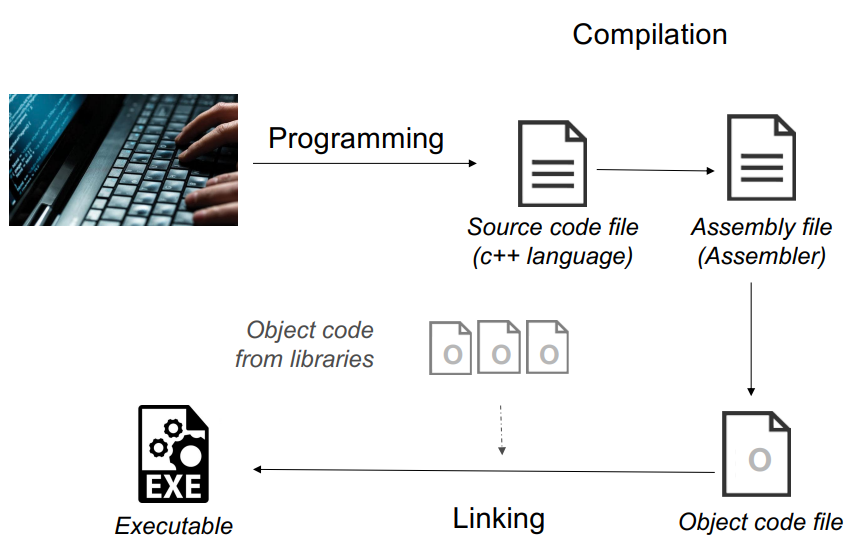
\includegraphics[scale=0.7]{figures/image1.png}
    \caption{Compilation and Linking}
    \label{fig:compilation_and_linking}
\end{figure}

The procedure is as follows:

\begin{itemize}
    \item The main file includes headers of the function/declarations it uses.
    \item Source files (.cpp) include the corresponding header (+ all headers for the functions/declarations they use).
    \item Source files are compiled separately and transformed (through the assembler!) into object code files.
    \item The linker merge together all object code files to build the executable.
\end{itemize}

\section{Classes and objects in \texttt{C++}}

Classes and objects are used to represent real-world entities in a program. They allow you to define the properties and
behaviors of an entity, and then create instances of the entity in the program. Classes are used to define the structure
of an entity, while objects are used to create instances of the entity.\\

A class is a (used-defined) data type that specifies how objects of its type can be created and used. A class directly 
represents a concept in a program. In \texttt{C++}, as in most modern languages, a class is the key building block for
large programs. Classes implement a very important concept: Abstract Data Types (ADTs).\\

An Abstract Data Type (ADT) is a data type that is defined by its behavior (its methods) rather than its implementation
(its data members). An ADT is a high-level view of a data type that specifies what operations can be performed on the data
type, but not how they are implemented. It offers a simple interface to the user, hiding the details of the implementation.
This is known as data encapsulation.\\

A class is an ADT characterized by:

\begin{itemize}
    \item Interface (public part): The interface of a class is the set of operations that can be performed on the objects 
    of the class.
    \item Implementation (private part): The implementation of a class is the set of data members and methods that are used 
    to implement the operations of the class.
\end{itemize}

An object is an instance of a class. It is a concrete realization of the class, with its own data members and methods. An
object is created by instantiating a class, which means allocating memory for the object and initializing its data members.\\

Let us take a look at the following code:

\begin{lstlisting}[language=C++]
\\stack.h
#ifndef STACK_H
#define STACK_H

class Stack {
public:
    Stack(int size);
    ~Stack();
    void push(int value);
    int pop();
    bool is_empty();
    bool is_full();
private:
    int* data;
    int size;
    int top;
};

#endif
\end{lstlisting}

\begin{lstlisting}[language=C++]
\\stack.cpp
#include "stack.h"

Stack::Stack(int size) {
    data = new int[size];
    this->size = size;
    top = -1;
}

Stack::~Stack() {
    delete[] data;
}

void Stack::push(int value) {
    if (!is_full()) {
        top++;
        data[top] = value;
    }
}

int Stack::pop() {
    int value = -1;
    if (!is_empty()) {
        value = data[top];
        top--;
    }
    return value;
}

bool Stack::is_empty() {
    return top == -1;
}

bool Stack::is_full() {
    return top == size - 1;
}
\end{lstlisting}

\begin{lstlisting}[language=C++]
\\main.cpp
#include <iostream>
#include "stack.h"
using namespace std;

int main() {
    Stack stack(3);
    stack.push(1);
    stack.push(2);
    cout << "pop: " << stack.pop() << endl;
    cout << "pop: " << stack.pop() << endl;
    return 0;
}

// Output:
// pop: 3
// pop: 2
\end{lstlisting}

In this code, we are defining a class called \texttt{Stack} that represents a stack data structure. The class contains
four public methods: \texttt{push}, \texttt{pop}, \texttt{is\_empty}, and \texttt{is\_full}. The class also contains
three private data members: \texttt{data}, \texttt{size}, and \texttt{top}. We are then defining the methods of the
class in the \texttt{stack.cpp} file. We are then using the class in the \texttt{main.cpp} file. Note that the class
definition is in the header file, while the class implementation is in the source file.\\

\section{Vectors}

Vectors are a sequence container that encapsulates dynamic size arrays. They can resize themselves automatically when
inserting elements. To use a vector, you need to include the \texttt{vector} header file.\\

A vector is a class template, which means that you can create vectors of any assignable type. It is provided by the Standard Template
Library (STL), which is a collection of classes and functions that are used to implement common data structures and algorithms.
Templates are not themselves classes or functions, but they instead can be thought of as the instructions to the compiler for 
generating classes or functions. This process is called instantiation.\\

Let us take a look at the following code:

\begin{lstlisting}[language=C++]
#include <iostream>
#include <vector>
using namespace std;

int main() {
    vector<int> numbers;
    numbers.push_back(1);
    numbers.push_back(2);
    numbers.push_back(3);
    for (int i = 0; i < numbers.size(); i++) {
        cout << "numbers[" << i << "] = " << numbers[i] << endl;
    }
    return 0;
}

// Output:
// numbers[0] = 1
// numbers[1] = 2
// numbers[2] = 3
\end{lstlisting}

In this code, we are creating a vector called \texttt{numbers} that can store integer values. We are then adding the values
1, 2, and 3 to the vector using the \texttt{push\_back} method. We are then using a \texttt{for} loop to iterate over the
vector and print the values to the console.\\

\subsection{Ways to initialize a vector}

There are several ways to initialize a vector in \texttt{C++}:\\

\begin{table}[ht]
\centering
\begin{tabular}{|l|p{7cm}|}
\hline
\texttt{vector <T> v1} & Vector that holds objects of type \texttt{T}. Default initialization, \texttt{v1} is empty \\
\hline
\texttt{vector <T> v2(v1)} & \texttt{v2} has a copy of each element in \texttt{v1} \\
\hline
\texttt{vector <T> v2 = v1} & As above \\
\hline
\texttt{vector <T> v3(n, val)} & \texttt{v3} has \texttt{n} elements with value \texttt{val} \\
\hline
\texttt{vector <T> v4(n)} & \texttt{v4} has \texttt{n} copies of a value-initialized object \\
\hline
\texttt{vector <T> v5 = }\{\texttt{a, b, c,...}\} & \texttt{v5} has as many elements as there are initializers; elements are initialized by corresponding initializers \\
\hline
\texttt{vector <T> v5 = }\{\texttt{a, b, c,...}\} & As above \\
\hline
\end{tabular}
\caption{Vector Initialization in C++}
\label{tab:vector_init}
\end{table}

Note that we can only create vectors that contain values with assignable types.
That is, values that can be reassignable throughout the code. Types like references
and \texttt{const} are non-assignable, so they cannot be used to construct vectors.\\

Vectors grow efficiently, and because of this, it is often unnecessary to specify the size of a vector when it is created,
since it can lead to poorer performance. The exception of this is when you know the size of the vector in advance.\\

The fact that we can easily and efficiently add elements to a vector is one of the reasons why vectors are so popular in
\texttt{C++}, since it greatly simplifies many programming tasks. This simplicity imposes a new obligation on the programmer:
we must ensure that any loops we write are correct, even if the loop changes the size of the vector.\\

\subsection{Summary of Vectors operations}

\begin{table}[ht]
\centering
\begin{tabular}{|l|p{7cm}|}
\hline
\textbf{Operation} & \textbf{Description} \\
\hline
\texttt{v.empty()} & Returns true if \texttt{v} is empty, false otherwise \\
\hline
\texttt{v.size()} & Returns the number of elements in \texttt{v} \\
\hline
\texttt{v.push\_back(t)} & Adds a new element with value \texttt{t} to the end of \texttt{v} \\
\hline
\texttt{v[n]} & Returns a reference to the element at position \texttt{n} in \texttt{v} \\
\hline
\texttt{v1 = v2} & Replaces the elements in \texttt{v1} with a copy of the elements in \texttt{v2} \\
\hline
\texttt{v1 == v2} & Returns true if \texttt{v1} and \texttt{v2} have the same size and the elements in corresponding positions are equal, false otherwise \\
\hline
\texttt{v1 != v2} & Returns true if \texttt{v1} and \texttt{v2} have different sizes or the elements in corresponding positions are not equal, false otherwise \\
\hline
\texttt{<, <=, >, >=} & Lexicographical comparison of \texttt{v1} and \texttt{v2} \\
\hline
\end{tabular}
\caption{Vector Operations in C++}
\label{tab:vector_operations}
\end{table}





